\documentclass{article}
\usepackage{tenor2015}
\usepackage{times}
\usepackage{ifpdf}
\usepackage[english]{babel}
\usepackage{cite}

\usepackage{inconsolata}
\usepackage{verbatim}

\usepackage{listings}
\lstset{language=Python,
showspaces=false,
showtabs=false,
breaklines=false,
showstringspaces=false,
breakatwhitespace=false,
escapeinside={(*@}{@*)},
keywordstyle=\bfseries,
basicstyle=\scriptsize\ttfamily
}

\def\papertitle{Design Priorities in Abjad:
    A Python API for Formalized Score Control}
\def\firstauthor{Trevor Ba\v{c}a}
\def\secondauthor{Josiah Wolf Oberholtzer}
\def\thirdauthor{Jeffrey Trevi\~{n}o}
\def\fourthauthor{V\'{i}ctor Ad\'{a}n}

\newif\ifpdf
\ifx\pdfoutput\relax
\else
   \ifcase\pdfoutput
      \pdffalse
   \else
      \pdftrue
\fi

\ifpdf % compiling with pdflatex
  \usepackage[pdftex,
    pdftitle={\papertitle},
    pdfauthor={\firstauthor, \secondauthor, \thirdauthor, \fourthauthor},
    bookmarksnumbered, % use section numbers with bookmarks
    pdfstartview=XYZ % start with zoom=100% instead of full screen; 
                     % especially useful if working with a big screen :-)
   ]{hyperref}
  %\pdfcompresslevel=9

  \usepackage[pdftex]{graphicx}
  % declare the path(s) where your graphic files are and their extensions so 
  %you won't have to specify these with every instance of \includegraphics
  \graphicspath{{./figures/}}
  \DeclareGraphicsExtensions{.pdf,.jpeg,.png}

  \usepackage[figure,table]{hypcap}

\else % compiling with latex
  \usepackage[dvips,
    bookmarksnumbered, % use section numbers with bookmarks
    pdfstartview=XYZ % start with zoom=100% instead of full screen
  ]{hyperref}  % hyperrefs are active in the pdf file after conversion
  \usepackage[dvips]{epsfig,graphicx}
  \graphicspath{{./figures/}}
  \DeclareGraphicsExtensions{.eps}
  \usepackage[figure,table]{hypcap}
\fi

\hypersetup{
    colorlinks,
    citecolor=black,
    filecolor=black,
    linkcolor=black,
    urlcolor=black
}

\title{\papertitle}

\fourauthors
  {\firstauthor} {Harvard University \\
    {\tt \href{mailto:trevor.baca@gmail.com}
        {trevor.baca@gmail.com}}}
  {\secondauthor} {Harvard University \\
    {\tt \href{mailto:josiah.oberholtzer@gmail.com}
        {josiah.oberholtzer@gmail.com}}}
  {\thirdauthor} {Carleton College \\
    {\tt \href{mailto:jeffrey.trevino@gmail.com}
        {jeffrey.trevino@gmail.com}}}
  {\fourthauthor} { 
    {\tt \href{mailto:vctradn@gmail.com}
        {vctradn@gmail.com}}}

\begin{document}

\capstartfalse
\maketitle
\capstarttrue

\begin{abstract}
Abjad\footnote{www.projectabjad.org} is an interactive open-source software
system designed to help composers build up complex pieces of music notation in
an iterative and incremental way.  Abjad is implemented in the
Python\footnote{www.python.org} programming language and architected as an
object-oriented collection of packages, classes and functions. Composers can
visualize their work as publication-quality score at all stages of the
compositional process using Abjad's interface to the
LilyPond\footnote{www.lilypond.org} music notation package. Although the first
versions of Abjad were implemented in 1997 and the project website is now
visited thousands of times each month, we have never documented the design
priorities that have guided us as we have built the system. In this paper we
detail some of the most important principles we have followed in our work
architecting Abjad. The priorities we document here arise in answer to
domain-specific questions of music modeling (what are the fundamental elements
of music notation? which elements of music notation should be modeled
hierarchically? which programming constructs are available to help model the
temporal relationships arising between entities in musical score?) as well as
in consideration of the ways in which best practices taken from software
engineering can apply to the development of a music software system like ours
(which programming concepts concerning things like iteration, aggregation and
encapsulation make sense to make available to composers? which existing tools
to test, document and deploy other open-source projects are available to help
develop a music software system like Abjad?). In the sections that follow we
discuss the background and motivations that lead us to ask questions like these
and then elaborate the design priorities we have arrived at in our ongoing work
architecting Abjad.
\end{abstract}

\section{Background \& Motivations}\label{sec:background}

While many environments for both notation and sound production have arisen
within the last twenty years, the following discussion focuses solely on the
production of notation: Abjad enables composers to express both low- and
high-level compositional ideas by extending a widely used programming language
to provide a sufficiently detailed object model of common practice musical
notation. To minimize the restriction of artistic thought's infinite
possibility while maximizing the ability to specify elegantly any arbitrary
symbolic relationship, Abjad does this without prescribing explicit or implicit
models of music or composition: Abjad defines composition narrowly as the act
of creating a document via the encoded aggregation of notational symbols.

\subsection{Generative Task as an Analytic Framework}

Software production exists as an organizationally designed feedback loop
between production values and implementation \cite{Derniame:1999fk}, and it is
possible to understand a system by understanding the purpose for which it was
initially designed, the system's \emph{generative task(s)}. In the analysis of
systems created for use by artists, this priority yields a dilemma instantly,
as analyses that explain a system's affordances with reference to intended
purpose must contend with the creative use of technology by artists: a system's
intended uses might have little or nothing in common with the way in which the
artist finally uses the technology. For this reason, the notion of generative
task is best understood as an explanation for a system's affordances, with the
caveat that a user can nonetheless work against those affordances to use the
system in novel ways. Generative tasks --- informed by the cultural milieu of
software development, economic constraints of software production, and the
aesthetic proclivities of artists participating in development processes ---
constrain software features to enable a limited subset of possible
representations and user interactions.

While composers working traditionally may allow intuition to substitute for
formally defined principles, a computer demands the composer to think formally
about music \cite{Xenakis:1992rq}. Keeping in mind generative task as an
analytical framework, it is broadly useful to bifurcate an automated notation
system's development into the modeling of music and composition, on the one
hand, and the modeling of musical notation, on the other. All systems model
both, to greater or lesser degrees, often engaging in the ambiguous or implicit
modeling of music and composition while focusing more ostensibly on a model of
notation, or focusing on the abstract modeling of music without a considered
link to a model of notation. Due to the intimate link between notation and
musical ideas, it is impossible for a system that models notation to avoid at
least implicitly modeling musical and compositional ideas, and a computational
model of music and composition is an inevitable component of every automated
notation system, even when it exists as an unspoken set of technological
constraints. Generative task explains a given system's balance between
computational models of music/composition and notation by assuming a link
between intended use and system development.

\subsection{Computational Models of Notation}

Many systems implement detailed models of music explicitly or implicitly, but
few of these implement detailed models of notation.\footnote{Computational
models of music might entail the representation of higher-level musical
entities apparent in the acts of listening and analysis but absent in the
symbols of notation themselves, as determined to be creatively exigent.
Programming researchers and musical artists have modeled many such
extrasymbolic musical entities, such as large-scale form and transition
\cite{polansky1991morphological}, \cite{uno1994temporal},
\cite{dobrian1995algorithmic}, \cite{abrams1999higher}, \cite{Yoo1983}, texture
\cite{Horenstein:2004kx}, contrapuntal relationships \cite{Boenn:2009oq},
\cite{Acevedo2005}, \cite{Anders:2011kl}, \cite{Balser:1990tg},
\cite{Jones:2000hc}, \cite{uno1994temporal}, \cite{Bell:1995ij},
\cite{farbood2001analysis}, \cite{Cope:2002fv}, \cite{Laurson:2005dz},
\cite{Polansky:2011fu}, \cite{Ebcioglu:1980kl}, harmonic tension and resolution
\cite{Melo2003}, \cite{Wiggins1999}, \cite{Foster:1995qa}, melody
\cite{Hornel:1993mi}, \cite{Smith:1992pi}, meter \cite{Hamanaka:2005ff}, rhythm
\cite{Nauert2007}, \cite{Degazio:1996lh}, \cite{Collins:2003bs}, timbre
\cite{Xenakis:1991fu}, \cite{Creasey:1996ye}, \cite{Osaka2004}, temperament
\cite{Seymour:2007qo}, \cite{Graf:2006il}, and ornamentation
\cite{Ariza:2003zt}, \cite{Chico-Topfer:1998jl}. This work overlaps fruitfully
with analysis tasks, and models of listening and cognition can enable novel
methods of high-level musical structures and transformations, like dramatic
direction, tension, and transition between sections \cite[108]{Collins2009}.} A
system that affords a detailed model of music/composition without linking to a
sufficiently detailed model of musical notation does not afford automated
notation --- sufficiency, however, depends heavily on generative task. For
example, if a composer requires an automated notation system to render complex
rhythmic ideas that depend typographically on nested tuplets, a system that
produces a notation only via a combination of MIDI and quantization must reduce
rhythms to a non-hierarchical stream of event times, eliminating the temporally
divisive approach of tuplet notation. For many rhythmic applications, though,
MIDI suffices. 

Many automated notation systems exist to model musical notation and the act of
typographical layout without explicitly affording the computational modeling of
music or composition \cite{Smith:1972mw}, \cite{Nienhuys:2003ve},
\cite{Hoos:1998bd}, \cite{hamel1noteability}; many of these systems strongly
imply a model of music, such as Gr\'{e}goire for Gregorian chant, Django for
guitar tablature, and GOODFEEL for Braille notation \cite{2006}, while
feature-rich systems (often oriented toward classical composers) such as
Finale, Sibelius, SCORE, Igor, Berlioz, and Nightingale, present themselves as
relatively more genre-agnostic software tools. Such a system might go so far as
to enable a text-based object-oriented model of notation that automates some
aspect of an otherwise point-and-click interface, as in the case of Sibelius's
ManuScript scripting language \cite{Technology:qc}. 

Many models of musical notation have been designed created for purposes of
corpus-based computational musicology. Formats such as Music21, DARM, SMDL,
HumDrum, and MuseData model notation with the generative task of searching
through a large amount of data \cite{Selfridge-Field:1997ud}. Commercial
notation software developers attempted to establish a data interchange standard
for optical score recognition (NIFF) \cite{niff1995niff}; since its release in
2004, MusicXML has become a valid interchange format for over 160 applications
and maintains a relatively application-agnostic status, as it was designed with
the generative task of acting as an interchange format between variously tasked
systems \cite{Good:2001if}. (are Igor and Berlioz commercial?)

Notation representations that underly many of these GUI-based systems often go
undescribed as computer representations of notation, in favor of discussions
about human-computer interaction. For example, Barker and Cantor developed an
early model of music notation that underlies a four-oscilloscope GUI and
describe their work entirely in terms of user interaction
\cite{cantor1971computer}; likewise, discussions of modern commercial notation
systems remain similarly oriented, without much awareness or criticism of the
underlying computational models of notation. This results in insufficiently
detailed models of notation; systems, for example, that provide models only of
mensural notation and enable nonmensural notations only as modified
instantiations of notations based on measures.

\subsection{The Development of Hierarchical Object Models of Notation}

Many early models of musical notation were not hierarchical, and Lejaran
Hiller, in reflecting on decades of automated notation work, identifies the
lack of hierarchical organization as a limitation of early work --- although
Nick Collins points out that even Hiller's program PHRASE addresses the
hierarchical organization of a score up to the level of a phrase, without
moving beyond this mid-level musical structure to concerns of large-scale form
\cite[108]{Collins2009}. 

There were several object-oriented music environments by 1990
\cite[139]{Polansky:1990fk}, most created in or inspired by the newly popular
Smalltalk-80 programming language; while they facilitated the hierarchical
modeling of musical abstractions, they omitted or radically simplified the
hierarchical nature of common notation. For example, Glen Krasner (Xerox
Systems Science Laboratory) created Machine Tongues VIII, a music system that
created an object-oriented model of the score/orchestra distinction inherited
from Max Mathews' Music N languages, with a simple linear model of ``partOn''
and ``partOff'' command sequences \cite{Krasner:1991uq}, omitting hierarchical
organization entirely when the system produced notational output; although
subsequent Machine Tongues systems introduced some hierarchical organization
via ``note'' objects that inhabited ``event lists,'' systems did not attempt to
model the hierarchical detail of all a traditional score's elements. Like
Hiller's PHRASE program, Andreas Mahling's CompAss system organized events
hierarchically up to the mid-level ``phrase'' level of musical structure
\cite{Mahling:1991qf}. These systems extend Smalltalk-80 with interfaces to the
MIDI communications protocol: as extensions of Smalltalk, they enabled the user
to arbitrarily extend the system with new objects, creating a detailed and
hierarchical model of music, usually flattened into a list of noteOn and
noteOff commands to be notated or played back via MIDI interface. 

By 1989, Glendon Diener's Nutation system (written in Objective C for the NeXT
computer) modeled both musical and notational structure hierarchically through
the use of directed graphs \cite{Diener:1991zr}, \cite{Diener:1991ly},
\cite{Diener:1989ve}.

last section: system motivations

Linking our design priorities with those of previous systems by describing
perceived deficiencies: evaluative priorities for previous systems: sufficiency
instead of comprehensiveness, potentially evaluated by sonic result rather than
notation, addressability (in HMSL and JMSL). Reintroduce generative task: late
50s through 80s were motivated locally by generative tasks of specific projects
until IRCAM's Patchwork approached a generative task of broadly enabling
composers; sufficiency determined by comprehensive task.
\section{Notational isomorphism}\label{sec:notational_isomorphism}

The set of typographical notation symbols overlaps with the set of
extrasymbolic musical entities, often causing confusion in discourse and
program architecture.\footnote{A ``chord'', for example, might be a vertically
ordered collection of pitch-classes in a harmonic conceit, or it might refer to
the specific arrangement of pitched note heads, stemmed together into a
composite notation symbol that instructs a performer to perform a sound that
consists of several component pitches.} Because of conceptual overlap between
music and notation, it can be difficult to separate a system’s model of
music/composition from its model of notation.

Abjad handles this ambiguity by explicitly modeling symbols on the page
according to common practice notation.

We provide one class per musical/typographic construct, such as \texttt{Note},
\texttt{NoteHead}, \texttt{Chord}, \texttt{Rest}, \texttt{Slur},
\texttt{Articulation} and so forth.

A \texttt{Note} object has one \texttt{NoteHead}, while a \texttt{Chord}
contains a collection of \texttt{NoteHead} objects.

Components:

\begin{lstlisting}
>>> score = Score()
>>> staff_group = StaffGroup()
>>> upper_staff = Staff(name='Upper Staff')
>>> outer_tuplet_one = Tuplet((2, 3), "d''16 ef'8.")
>>> inner_tuplet = Tuplet((4, 5), "cs''16 e'16 d'2")
>>> outer_tuplet_one.append(inner_tuplet)
>>> outer_tuplet_two = Tuplet((4, 5), "d'8 r16 b'16 as'16")
>>> upper_staff.extend([outer_tuplet_one, outer_tuplet_two])
>>> upper_staff.extend("as'8.. fs'32")
>>> lower_staff = Staff(name='Lower Staff')
>>> lower_staff.extend("c8 r8 b8 r8 gf8 r4 cs8")
>>> staff_group.extend([upper_staff, lower_staff])
>>> score.append(staff_group)
>>> show(score)
\end{lstlisting}

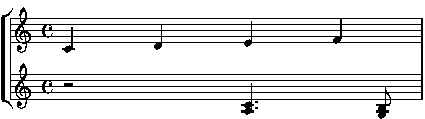
\includegraphics[scale=1.0]{images/notational_isomorphism-1.pdf}


Spanners:

\begin{lstlisting}
>>> upper_leaves = upper_staff.select_leaves()
>>> attach(Tie(), upper_leaves[4:6])
>>> attach(Tie(), upper_leaves[-3:-1])
>>> attach(Slur(), upper_leaves[:2])
>>> attach(Slur(), upper_leaves[2:6])
>>> attach(Slur(), upper_leaves[7:])
>>> show(score)
\end{lstlisting}

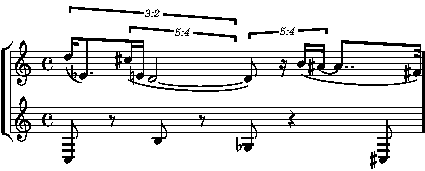
\includegraphics[scale=1.0]{images/notational_isomorphism-2.pdf}


Indicators:

\begin{lstlisting}
>>> attach(Dynamic('f'), upper_leaves[0])
>>> attach(Dynamic('p'), upper_leaves[-4])
>>> attach(Articulation('accent'), upper_leaves[0])
>>> attach(Articulation('accent'), upper_leaves[2])
\end{lstlisting}


\begin{lstlisting}
>>> lower_leaves = lower_staff.select_leaves()
>>> attach(Clef('bass'), lower_leaves[0])
>>> for note in iterate(lower_staff).by_class(Note):
...     attach(Articulation('staccato'), note)
... 
>>> show(score)
\end{lstlisting}

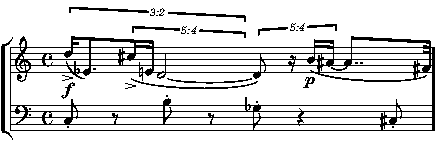
\includegraphics[scale=1.0]{images/notational_isomorphism-3.pdf}


\subsection{Building up score: iterative aggregation}

Abjad assumes notational primitives are the elements of composition. The act of
composition then revolves around the iterative aggregation of notational
primitives into arbitrarily complex score objects. Abjad affords aggregation
via Python's \emph{mutable sequence} protocol, a collection of instance methods
which allow score components to be appended, extended or inserted into other
container-like score components as though they were lists.

Spanners such as slurs, beams and glissandi and indicators such as
articulations and textual directions can be attached to score components via
the \texttt{attach()} function.

Abjad attempts to be compositionally agnostic. By providing simple and
unambiguous means of gradually aggregating arbitrarily complex score objects,
Abjad encourages users to develop their own personal approach.

\subsection{Modeling notation explicitly}

Abjad models notation explicitly. All notational primitives expressed by Abjad
must conform to the principles of common practice notation. When compositional
inputs cannot be expressed in terms of these principles, Abjad provides
affordances for massaging them into valid notational states.

For example, Abjad expresses the durations of all score components in terms of
rational values -- fractions and integers -- rather than floating point
numbers. Likewise Abjad expresses all pitches in terms of triples of diatonic
note names, accidentals and octave numbers, rather than MIDI numbers or
frequencies. While Abjad provides alternative representations of pitch and
rhythm, as well as affordances for moving between them, the format actually
stored in and used by score components for rendering notation is always the
most notationally-explicit.

%\subsection{Written, assignable and prolated durations}

All \texttt{Note}, \texttt{Chord} and \texttt{Rest} objects in Abjad must be
instantiated with a duration corresponding to the written glyphs on the page --
a \emph{written} duration.

Written durations must be \emph{assignable}, a category we invented to model
durational initialization. Durational assignability describes whether a
duration can be represented as a power-of-two flag count combined with zero or
more dots. \texttt{1/4}, \texttt{3/16} and \texttt{7/16} are assignable
durations while \texttt{5/32}, \texttt{9/8} and \texttt{1/12} are not.

Non-assignable durations cannot be represented in common practice notation by a
single glyph. They require two or more glyphs with assignable durations tied
together, for the score component to be tupletted, or both.

Abjad will not automatically render a single note with a duration of
\texttt{5/16} as two or more notes tied together. We consider such behavior to
be too implicit. There are too many potentially compositionally valid ways to
render a duration such as \texttt{5/16} into a series of tied assignable
durations: \texttt{1/4 + 1/16}, \texttt{3/16 + 2/16}, \texttt{2/16 + 3/16},
\texttt{1/16 + 1/4}, \texttt{1/8 + 1/8 + 1/16} etc. Instead we provide
affordances for generating tied notes from non-assignable durations. One such
affordance is our \texttt{scoretools.make\_notes()} function, which chooses
smart defaults for generating tied glyphs from otherwise un-notateable input.

\begin{lstlisting}
>>> selection = scoretools.make_notes("c'", [(5, 16)])
>>> staff = Staff(selection)
>>> show(staff)
\end{lstlisting}

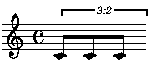
\includegraphics[scale=1.0]{images/notational_isomorphism-4.pdf}


All score components also have a \emph{prolated} duration - the product of
their written duration and their \emph{prolation}. Prolation is the cumulative
product of all the \emph{multiplier} of every tuplet found in the
\emph{parentage} of a score component. A score component's prolation depends on
its location in the score hierarchy, and is not an inherent property of itself
independent that hierarchy.

Three \texttt{Note} objects each having a prolated duration of \texttt{1/12}
can be represented as either three \texttt{1/16} notes in a \texttt{3:4} tuplet
or as three \texttt{1/8} notes in a \texttt{3:2} tuplet. As all Abjad
\texttt{Note} objects must have an assignable written duration, the three notes
above must have written durations of either \texttt{1/8} or \texttt{1/16}, and
the tuplet must be correspondingly an explicit diminution or augmentation to
provide the desired prolation of \texttt{2/3} or \texttt{4/3}.

\begin{lstlisting}
>>> selection = scoretools.make_notes("c'", [(1, 12)] * 3)
>>> tuplet = selection[0]
>>> show(tuplet)
\end{lstlisting}

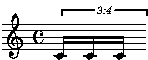
\includegraphics[scale=1.0]{images/notational_isomorphism-5.pdf}

\begin{lstlisting}
>>> tuplet.toggle_prolation()
>>> show(tuplet)
\end{lstlisting}

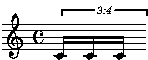
\includegraphics[scale=1.0]{images/notational_isomorphism-6.pdf}


The durational information of any aggregate score object in Abjad is therefore
always explicit and unambiguous with regard to its notational reality.
\section{Score Addressability}\label{sec:score_addressability}


\begin{comment}
Score Addressability [Trevor]
    - Iteration
        - methods that "get_*"
            Container.select_leaves
            Container.select_notes_and_chords
            IterationAgent.by_class, .by_logical_tie, .by_timeline, .by_vertical_moment, .depth_first
        - efficient and intuitive navigation of the score hierarchy does what mapping does in a functional program
            -containers partake of Python's sequence iterating interface (for loops work)
    - Structural Addressing
        - numeric addressing
        - temporal addressing
        - named addressing
\end{comment}

\subsection{Addressing objects by index}

Abjad allows the numeric addressing of all score components. Abjad score
components are zero-indexed from the start of the container which holds them:
the statement \texttt{staff[0]} addresses the first component contained in
\texttt{staff} while the statement \texttt{staff[1]} addresses the component
after that, and so on. Negative indices address components from the end of the
container which holds them. Python's slice notation may be used to retrieve an
arbitrary number of contiguous components at one time. As an example of the
latter, the statement \texttt{staff[15:25]} selects the ten components in
\texttt{staff} between indices 15 and 25. The conventions of Abjad's numeric
addressing regime follow those of Python's list and tuple interface exactly. 

\begin{lstlisting}
>>> staff_group = score[0]
\end{lstlisting}


\begin{lstlisting}
>>> upper_staff = score[0][0]
\end{lstlisting}


\begin{lstlisting}
>>> first_tuplet = score[0][0][0]
>>> show(first_tuplet)
\end{lstlisting}

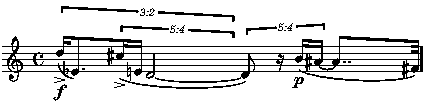
\includegraphics[scale=1.0]{images/score_addressability-1.pdf}


\subsection{Addressing objects temporally}

Here is some text.

A \emph{timespan} is an object-oriented model of a start/stop offset pair.
Abjad's \texttt{Timespan} class affords users with a variety of tests for
relationships between timespans such as overlap and intersection.

All durated objects in Abjad have a timespan, including all score components
and spanners, allowing them to partake in timespan-based relationship modeling
without regard for hierarchical score structure.

\subsection{Addressing objects by name}

Here is some text.

\begin{lstlisting}
>>> upper_staff = score['Upper Staff']
>>> show(upper_staff)
\end{lstlisting}

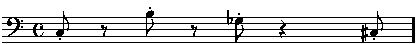
\includegraphics[scale=1.0]{images/score_addressability-2.pdf}


\begin{lstlisting}
>>> lower_staff = score['Lower Staff']
>>> show(lower_staff)
\end{lstlisting}

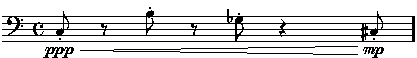
\includegraphics[scale=1.0]{images/score_addressability-3.pdf}


\subsection{Iterating throught score}

Here is some text.

\begin{lstlisting}
>>> for x in score['Upper Staff']:
...     x
... 
Tuplet(Multiplier(2, 3), 'd\'\'16 ef\'8. Tuplet(Multiplier(4, 5), "cs\'\'16 e\'16 d\'2 ~")')
Tuplet(Multiplier(4, 5), "d'8 r16 b'16 as'16 ~")
Note("as'8..")
Note("fs'32")
\end{lstlisting}


\begin{lstlisting}
>>> for component in iterate(score).by_timeline():
...     component
... 
Note("d''16")
Note('c8')
Note("ef'8.")
Rest('r8')
Note("cs''16")
Note("e'16")
Note("d'2")
Note('b8')
Rest('r8')
Note("d'8")
Note('gf8')
Rest('r16')
Rest('r4')
Note("b'16")
Note("as'16")
Note("as'8..")
Note('cs8')
Note("fs'32")
\end{lstlisting}


\begin{lstlisting}
>>> for logical_tie in iterate(score).by_logical_tie(
...     nontrivial=True,
...     pitched=True,
...     ):
...     logical_tie
... 
LogicalTie(Note("d'2"), Note("d'8"))
LogicalTie(Note("as'16"), Note("as'8.."))
\end{lstlisting}


\section{Relationship Modeling}\label{sec:relationship_modeling}

\subsection{Component, Spanner, Indicator}

Some text here.

Components:

\begin{lstlisting}
>>> staff = Staff()
>>> outer_tuplet_one = Tuplet((2, 3), "d''16 ef'8.")
>>> inner_tuplet = Tuplet((4, 5), "cs''16 e'16 d'2")
>>> outer_tuplet_one.append(inner_tuplet)
>>> outer_tuplet_two = Tuplet((4, 5), "d'8 r16 b'16 as'16")
>>> staff.extend([outer_tuplet_one, outer_tuplet_two])
>>> staff.extend("as'8.. fs'32")
>>> show(staff)
\end{lstlisting}

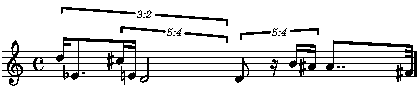
\includegraphics[scale=1.0]{images/relationship_modeling-1.pdf}


Spanners:

\begin{lstlisting}
>>> leaves = staff.select_leaves()
>>> attach(Tie(), leaves[4:6])
>>> attach(Tie(), leaves[-3:-1])
>>> attach(Slur(), leaves[:2])
>>> attach(Slur(), leaves[2:6])
>>> final_slur = Slur()
>>> attach(final_slur, leaves[7:])
>>> show(staff)
\end{lstlisting}

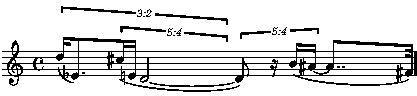
\includegraphics[scale=1.0]{images/relationship_modeling-2.pdf}


Indicators:

\begin{lstlisting}
>>> attach(Markup('giocoso', Up).italic(), leaves[0])
>>> attach(Markup('dolce', Up).italic(), leaves[-4])
>>> attach(Dynamic('f'), leaves[0])
>>> attach(Dynamic('p'), leaves[-4])
>>> attach(Articulation('accent'), leaves[0])
>>> attach(Articulation('accent'), leaves[2])
>>> show(staff)
\end{lstlisting}

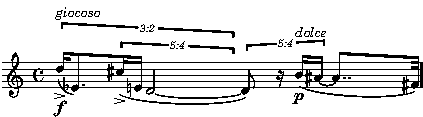
\includegraphics[scale=1.0]{images/relationship_modeling-3.pdf}


\subsection{Hierarchical relationships}

Abjad provides concrete object-models for various hierarchical relationships.

Leaves and parentage.

\begin{lstlisting}
>>> staff_leaves = staff.select_leaves()
>>> for leaf in staff_leaves:
...     leaf
... 
Note("d''16")
Note("ef'8.")
Note("cs''16")
Note("e'16")
Note("d'2")
Note("d'8")
Rest('r16')
Note("b'16")
Note("as'16")
Note("as'8..")
Note("fs'32")
\end{lstlisting}


\begin{lstlisting}
>>> tuplet_leaves = inner_tuplet.select_leaves()
>>> for leaf in tuplet_leaves:
...     leaf
... 
Note("cs''16")
Note("e'16")
Note("d'2")
\end{lstlisting}


\begin{lstlisting}
>>> third_note = staff_leaves[2]
>>> third_note
Note("cs''16")
\end{lstlisting}



\begin{lstlisting}
>>> parentage = inspect_(third_note).get_parentage()
>>> parentage.root
<Staff{4}>
\end{lstlisting}


\begin{lstlisting}
>>> parentage.tuplet_depth
2
\end{lstlisting}


\begin{lstlisting}
>>> parentage.prolation
Multiplier(8, 15)
\end{lstlisting}


\subsection{Temporal relationships}

Spanners.

Effective indicators.

Logical ties.

\begin{lstlisting}
>>> spanners = inspect_(leaves[0]).get_spanners(Slur)
>>> first_slur = tuple(spanners)[0]
>>> first_slur.components
Selection(Note("d''16"), Note("ef'8."))
\end{lstlisting}


\begin{lstlisting}
>>> for leaf in leaves:
...     dynamic = inspect_(leaf).get_effective(Dynamic)
...     print(dynamic, leaf)
... 
Dynamic(name='f') d''16
Dynamic(name='f') ef'8.
Dynamic(name='f') cs''16
Dynamic(name='f') e'16
Dynamic(name='f') d'2
Dynamic(name='f') d'8
Dynamic(name='f') r16
Dynamic(name='p') b'16
Dynamic(name='p') as'16
Dynamic(name='p') as'8..
Dynamic(name='p') fs'32
\end{lstlisting}


Logical ties.

\begin{lstlisting}
>>> for logical_tie in iterate(staff).by_logical_tie():
...     logical_tie
... 
LogicalTie(Note("d''16"),)
LogicalTie(Note("ef'8."),)
LogicalTie(Note("cs''16"),)
LogicalTie(Note("e'16"),)
LogicalTie(Note("d'2"), Note("d'8"))
LogicalTie(Rest('r16'),)
LogicalTie(Note("b'16"),)
LogicalTie(Note("as'16"), Note("as'8.."))
LogicalTie(Note("fs'32"),)
\end{lstlisting}


\section{Open Source}\label{sec:open_source}

\subsection{Compositional Agnosticism}

By providing core functionality oriented toward the elements of standard
notation, Abjad strives to remain as agnostic as possible to various
composition techniques. 

\subsection{Extensibility}

To better afford high-level, personal, eccentric composition techniques as
optional tools packages, Abjad provides clear examples of extensibility through
the authors' own included extensions, including: 

\begin{itemize}
    \item labeltools
    \item metertools
    \item quantizationtools
    \item rhythmmakertools
    \item selectortools
    \item sievetools
    \item tonalanalysistools
\end{itemize}

%\subsection{Affording Extension through Project Structure and Interface}

As an open-source project, composers and researchers can contribute changes via
git pull requests. A process of continuous integration and online version
control simplifies this contribution process. 

\subsection{Embeddability}

Abjad is an importable Python library. It can be used in whole or in part as a
component of any Python-compatible system. Abjad has few Python package
dependencies and is not bound to any specific user application or graphic user
interface. These qualities make Abjad an ideal project ideal for embedding in
other software systems.

For example, Abjad supports IPython
Notebook\footnote{http://ipython.org/notebook.html}, a web-based interactive
computational environment combining code execution, text, mathematics, plots
and rich media into a single document. Notational output from Abjad can be
transparently captured and embedded directly into an IPython Notebook which has
loaded Abjad's IPython Notebook extension. Calls to Abjad's \texttt{show()} are
intercepted and the rendered graphics are embedded directly into the Notebook
along with the generating code. This allows scholars to quickly and intuitively
create music texts which can be shared, edited and executed by other IPython
users.

\subsection{Testability}

Text here.

\subsection{Maintainability}

Text here.

%\begin{acknowledgments}
%You may acknowledge people, projects, 
%funding agencies, etc. 
%which can be included after the second-level heading
%``Acknowledgments'' (with no numbering).
%\end{acknowledgments} 

\bibliography{tenor2015}
\end{document}